In diesem Kapitel werden alle Grundlagen erläutert, welche nötig sind um den Versuch durchführen zu können. 

\subsection{Die Lichtgeschwindkeit}

An der Internationalen Konferenz für Mass und Gewicht kurz ICPM wurde der Meter durch Festlegung des Zahlenwertes für die Lichgeschwindigkeit im Vakuum wie folgt neu definiert.

%%%%%%%%%%%%%%%%%%%%%%%%%%%%%%%%%%%%%%%%%%%%%%%%%%%%%%%%%%%%%%%%%%%%%%%%%%%%%
\begin{equation*}
c_{0} = 299'792'458 m/s
\label{eq:Lichtgeschwindigkeit}
\end{equation*}
%%%%%%%%%%%%%%%%%%%%%%%%%%%%%%%%%%%%%%%%%%%%%%%%%%%%%%%%%%%%%%%%%%%%%%%%%%%%%

Die Lichtgeschwindigkeit in einem Medium wiederrum erhält man mit Hilfe des gemessenen Brechungsindexes $n$ definiert in Formel \ref{eq:Formel_Brechungsindex}. In einem Gas, also zum Beispiel in der Luft, ist $n$ proportional zur Dichte und wird noch durch die Luftfeuchtigkeit leicht beeinflusst.

%%%%%%%%%%%%%%%%%%%%%%%%%%%%%%%%%%%%%%%%%%%%%%%%%%%%%%%%%%%%%%%%%%%%%%%%%%%%%
\begin{equation}
c=c_{0}/n
\label{eq:Formel_Brechungsindex}
\end{equation}
%%%%%%%%%%%%%%%%%%%%%%%%%%%%%%%%%%%%%%%%%%%%%%%%%%%%%%%%%%%%%%%%%%%%%%%%%%%%%

Um den Brechungsindex $n$ auszurechnen, kann Formel \ref{eq:Formel_Brechungsindex_in_der_Luft} angewandt werden, wobei diese jedoch noch nach $n$ umgeformt werden muss.

%%%%%%%%%%%%%%%%%%%%%%%%%%%%%%%%%%%%%%%%%%%%%%%%%%%%%%%%%%%%%%%%%%%%%%%%%%%%%
\begin{equation}
(n - 1) = (n_{n} - 1)\cdot\dfrac{p \cdot T_{n}}{p_{n} \cdot T}-(\beta - \dfrac{\gamma}{\lambda}_{0}) \cdot p_{w}
\label{eq:Formel_Brechungsindex_in_der_Luft}
\end{equation}
%%%%%%%%%%%%%%%%%%%%%%%%%%%%%%%%%%%%%%%%%%%%%%%%%%%%%%%%%%%%%%%%%%%%%%%%%%%%%

Die in Formel \ref{eq:Formel_Brechungsindex_in_der_Luft} enthaltenen Parameter sind unteranderem die gemessene Raumtemperatur $T$ in Kelvin, sowie der gemessene Luftdruck $p$. $\beta$ und $\gamma$ sind Wasserdampfkorrekturfaktoren, sowie $\lambda_{0}$ die Vakuum-Wellenlänge, welche unmerklich verschwinden von der Luftwellenlänge ist, weshalb diese verwendet wird.

%%%%%%%%%%%%%%%%%%%%%%%%%%%%%%%%%%%%%%%%%%%%%%%%%%%%%%%%%%%%%%%%%%%%%%%%%%%%%
\begin{equation*}
\beta = 4.292 \cdot 10^{-8} mbar^{-1}
\label{eq:Faktor_Beta}
\end{equation*}
\begin{equation*}
\gamma = 3.43 \cdot 10^{-2} (nm)^{2}mbar^{-1}
\label{eq:Faktor_Gamma}
\end{equation*}
\begin{equation*}
\lambda_{0} = 632.8 nm
\label{eq:Faktor_Lambda}
\end{equation*}
%%%%%%%%%%%%%%%%%%%%%%%%%%%%%%%%%%%%%%%%%%%%%%%%%%%%%%%%%%%%%%%%%%%%%%%%%%%%%

Mit Hilfe der nachfolgenden Abbildung \ref{fig:Wasserdampfsättigung und Normbrechungsindex}, können die restlichen Parameter bestimmt werden. So kann beispielsweise aus der Abbildung links die p-Sättigung gelesen werden, anhand der gemessenen Raumtemperatur $T$ oder in der rechten Abbildung auf Grund der vorgegebenen Wellenlänge der Normbrechnungsindex $(n_{n} - 1)$ herausgelesen werden. Die restlichen Parameter $T_{n}$ und $p_{n}$ sind ebenfalls in der rechten Abbildung aus dem Text ablesbar und stellen die Parameter dar, auf welche die Abbildung rechts normiert ist.

%%%%%%%%%%%%%%%%%%%%%%%%%%%%%%%%%%%%%%%%%%%%%%%%%%%%%%%%%%%%%%%%%%%%%%%%%%%%%
\begin{figure}[b]
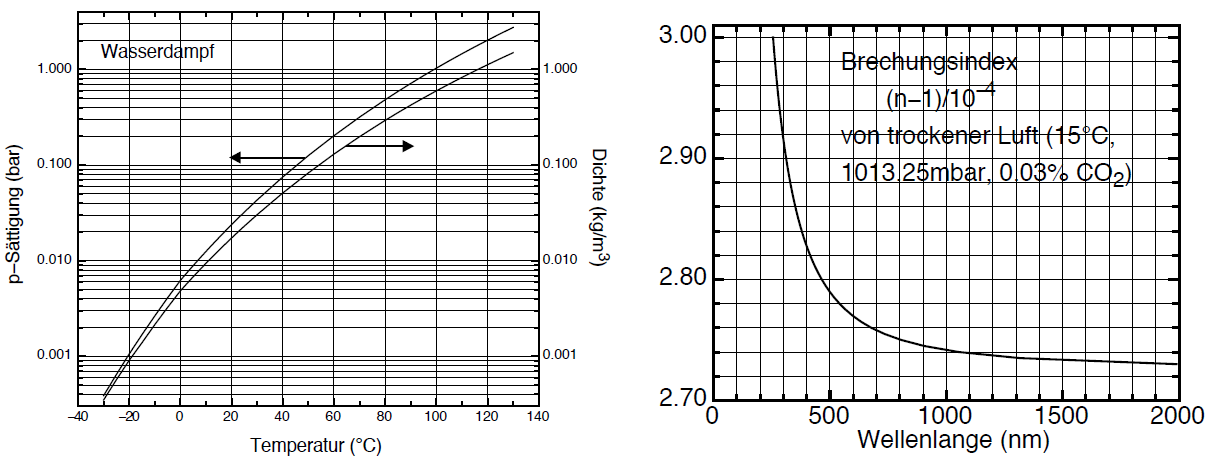
\includegraphics[width=\textwidth]{Brechungsindex_Luft_Grafik.png}
\caption{Wasserdampfsättigung und Normbrechungsindex}
\label{fig:Wasserdampfsättigung und Normbrechungsindex}
\end{figure}
%%%%%%%%%%%%%%%%%%%%%%%%%%%%%%%%%%%%%%%%%%%%%%%%%%%%%%%%%%%%%%%%%%%%%%%%%%%%%

Der Parameter $p_{w}$ wiederrum ist der Wasserdampfpartialdruck und wird separat mit Formel \ref{eq:Formel_Wasserdampfpartialdruck} ausgerechnet, wobei der aus Abbildung \ref{fig:Wasserdampfsättigung und Normbrechungsindex} gelesene Wert für die p-Sättigung verwendet wird, sowie die gemessene Luftfeuchtigkeit während der Versuchdurchführung.


%%%%%%%%%%%%%%%%%%%%%%%%%%%%%%%%%%%%%%%%%%%%%%%%%%%%%%%%%%%%%%%%%%%%%%%%%%%%%
\begin{equation}
p_{w} = \dfrac{Luftfeuchtigkeit}{100\%}\cdot p-Saettigung
\label{eq:Formel_Wasserdampfpartialdruck}
\end{equation}
%%%%%%%%%%%%%%%%%%%%%%%%%%%%%%%%%%%%%%%%%%%%%%%%%%%%%%%%%%%%%%%%%%%%%%%%%%%%%

Werden die aus Abbildung \ref{fig:Wasserdampfsättigung und Normbrechungsindex} ausgelesenen Werte und die restlich berechneten Werte in Formel \ref{eq:Formel_Brechungsindex_in_der_Luft} eingesetzt sowie nach $n$ aufgelöst, erhält man den spezifischen Brechungsindex $n$ der Versuchdurchführung. Dieser ermittelte Brechungsindex $n$, kann dann wiederrum in Formel \ref{eq:Formel_Brechungsindex} eingesetzt werden und man erhält den für die Versuchumgebung spezifische Wert der Lichtgeschwindigkeit $c$. 

\subsection{Messung der Lichtgeschwindigkeit nach Michelson}

Zur Bestimmung der Lichtgeschwindigkeit gibt es verschiendeste Methoden. Eine davon ist die Messung der Lichtgeschwindigkeit nach Michelson, welche die Funktion der Abbildung und Kollimation in einer langbrennweitigen Linse vereint. Dadurch kann erreicht werden, dass die Abbildungsqualität verbessert wird und man hat die Möglichkeit einer gewissen Freiheit bei der Wahl der Basisstrecke.

Um jedoch den Strahlengang verstehen zu können werden, werden noch die Abbildugnsgleichung sowie den Abbildungsmasstab $\beta$ benötigt.

%%%%%%%%%%%%%%%%%%%%%%%%%%%%%%%%%%%%%%%%%%%%%%%%%%%%%%%%%%%%%%%%%%%%%%%%%%%%%
\begin{equation}
\dfrac{1}{f} = \dfrac{1}{g} + \dfrac{1}{b}
\label{eq:Formel_Abbilungsgleichung}
\end{equation}
\begin{equation}
\beta = \frac{B}{G} = \frac{b}{g}
\label{eq:Formel_Abbildungsmassstab}
\end{equation}
%%%%%%%%%%%%%%%%%%%%%%%%%%%%%%%%%%%%%%%%%%%%%%%%%%%%%%%%%%%%%%%%%%%%%%%%%%%%%

In den Formeln \ref{eq:Formel_Abbilungsgleichung} und \ref{eq:Formel_Abbildungsmassstab} enthalten sind $f$ die Brennweite, $g$ die Gegenstandsweite, $b$ die Bildweite, $B$ die Bildgrösse und $G$ die Gegenstandsgrösse. Abbildung \ref{fig:Abbildung an einer Linse} zeigt die Anwendung dieser Formeln anhand einer Linse.

%%%%%%%%%%%%%%%%%%%%%%%%%%%%%%%%%%%%%%%%%%%%%%%%%%%%%%%%%%%%%%%%%%%%%%%%%%%%%
\begin{figure}[htb]
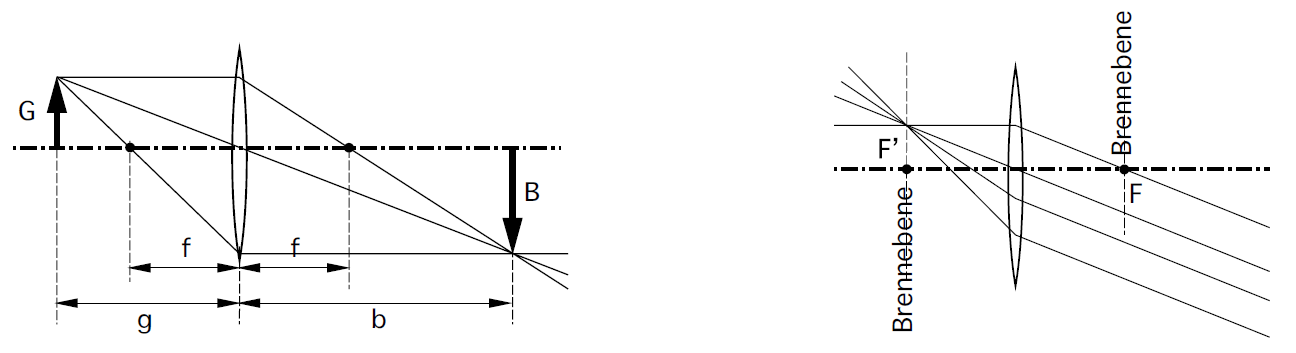
\includegraphics[width=\textwidth]{Abbildung_Linse_Grafik.png}
\caption{Abbildung an einer Linse}
\label{fig:Abbildung an einer Linse}
\end{figure}
%%%%%%%%%%%%%%%%%%%%%%%%%%%%%%%%%%%%%%%%%%%%%%%%%%%%%%%%%%%%%%%%%%%%%%%%%%%%%

Abbildung \ref{fig:Strahlengang Michelson} zeigt den Strahlengang. Als Messmarke dient anstatt eines Gitters ein einstellbarer vertikaler Spalt. Das an diesem Spalt leicht divergent auslaufende Licht wird durch die Linse $L_{1}$ abgebildet, wobei die Distanz zwischen Spalt und $L_{1}$ möglichst genau auf die Brennweite $f_{1}$ eingestellt werden muss. Der Drehspiegel DS wiederrum soll so justiert werden, dass das Licht auf die Mitte des Hohlspiegels HS trifft. Dieser Hohlspiegel HS bildet den Spalt in seine Brennebene ab, wo sich der Endspiegel ES befindet. Mit Hilfe des Strahlenteilers wird sodann das rückrefelektierte Bild im Messokular sichtbar.

%%%%%%%%%%%%%%%%%%%%%%%%%%%%%%%%%%%%%%%%%%%%%%%%%%%%%%%%%%%%%%%%%%%%%%%%%%%%%
\begin{figure}[htb]
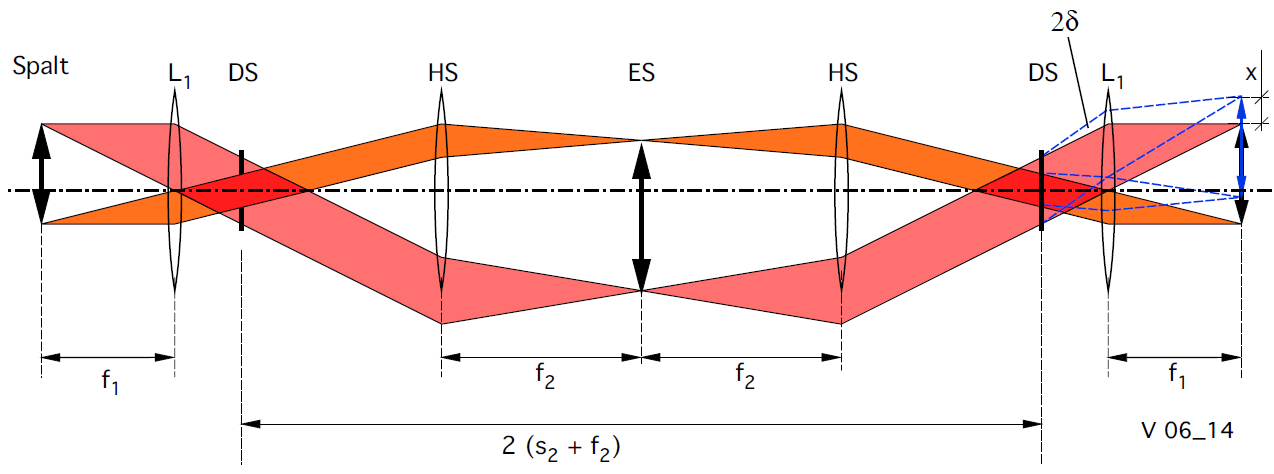
\includegraphics[width=\textwidth]{Strahlengang_Michelson_Grafik.png}
\caption{Strahlengang Michelson}
\label{fig:Strahlengang Michelson}
\end{figure}
%%%%%%%%%%%%%%%%%%%%%%%%%%%%%%%%%%%%%%%%%%%%%%%%%%%%%%%%%%%%%%%%%%%%%%%%%%%%%

Bei einem sich rotierenden Spiegel findet das vom Endspiegel ES zurückkehrende Licht den Drehspiegel um einen Winkel $\delta$ gedreht. Daher gilt nachfolgende Formel \ref{eq:Formel_Winkeländerung}.

%%%%%%%%%%%%%%%%%%%%%%%%%%%%%%%%%%%%%%%%%%%%%%%%%%%%%%%%%%%%%%%%%%%%%%%%%%%%%
\begin{equation}
\delta = \omega\cdot\Delta t = \omega\cdot\dfrac{2\cdot(s_{2}+f_{2})}{c}
\label{eq:Formel_Winkeländerung}
\end{equation}
%%%%%%%%%%%%%%%%%%%%%%%%%%%%%%%%%%%%%%%%%%%%%%%%%%%%%%%%%%%%%%%%%%%%%%%%%%%%%

In Formel \ref{eq:Formel_Winkeländerung} enthalten ist die Kreisfrequenz $\omega$ des Drehspiegels, und $\Delta t$ die Laufzeit des Lichtes vom Drehspiegel zum Endspiegel und zurück. Genau diese Drehung des Speigels führt zu einer Richtungsänderung der Bündelachse um den Winkel $2\delta$ und damit auch zu einer seitlichen Verschiebung x wie in Abbildung \ref{fig:Strahlengang Michelson} ersichtlich ist.\\
Durch die mit Formel \ref{eq:Formel_Kleinwinkelnäherung_Michelson} angewendete Kleinwinkelnäherung ergibt sich schliesslich die gesuchte Formel \ref{eq:Formel_Lichtgeschwindigkeit_Michelson} zur Bestimmung der Lichgeschwindigkeit $c$ nach der Michelson Methode.

%%%%%%%%%%%%%%%%%%%%%%%%%%%%%%%%%%%%%%%%%%%%%%%%%%%%%%%%%%%%%%%%%%%%%%%%%%%%%
\begin{equation}
2\cdot\delta = x/f_{1}
\label{eq:Formel_Kleinwinkelnäherung_Michelson}
\end{equation}
%%%%%%%%%%%%%%%%%%%%%%%%%%%%%%%%%%%%%%%%%%%%%%%%%%%%%%%%%%%%%%%%%%%%%%%%%%%%%

%%%%%%%%%%%%%%%%%%%%%%%%%%%%%%%%%%%%%%%%%%%%%%%%%%%%%%%%%%%%%%%%%%%%%%%%%%%%%
\begin{equation}
c = 4\cdot\omega\cdot\dfrac{(s_{2}+f_{2})\cdot f_{1}}{x}
\label{eq:Formel_Lichtgeschwindigkeit_Michelson}
\end{equation}
%%%%%%%%%%%%%%%%%%%%%%%%%%%%%%%%%%%%%%%%%%%%%%%%%%%%%%%%%%%%%%%%%%%%%%%%%%%%%


